%----------------------------------------------------------
%
\documentclass[xcolor=dvipsnames]{beamer}%

\mode<presentation> {
  \usetheme{CambridgeUS}
  \usefonttheme[onlymath]{serif}
  \setbeamercovered{transparent}
}

\usepackage{hyperref}

\hypersetup{colorlinks,linkcolor=,urlcolor=blue}
\usepackage{minted}
\usepackage{multicol}
%\usepackage{utf-8}

\setbeamertemplate{itemize item}{\raisebox{0.25ex}{\small\textbullet}}
\setbeamertemplate{itemize subitem}{\raisebox{0.25ex}{\scriptsize\textbullet}}
\graphicspath{{figures/}}
\logo{\resizebox{10mm}{!}{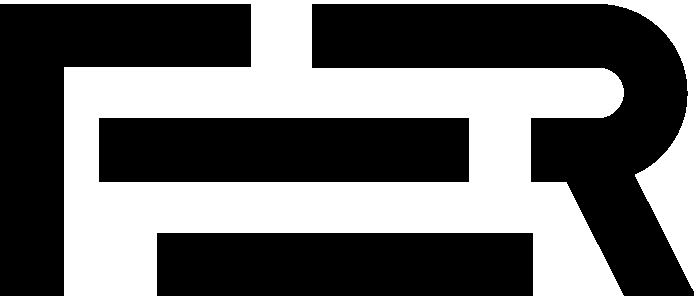
\includegraphics{FER_logo}}}
\setbeamersize{text margin left=15pt, text margin right=20pt} 
\setlength{\leftmarginii}{10pt}
\setbeamertemplate{enumerate item}{
    \raisebox{-1.7pt}{\scalebox{2.1}{\textbullet}\hskip-14.3pt}
    \hbox to2ex{%
      \hfil
      \usebeamercolor[bg]{item projected}
      \color{fg}
      \raisebox{1.7pt}{\scalebox{0.65}{\insertenumlabel}}%
      \hfil}
    \hskip-5pt%
}
\setbeamertemplate{section in toc}{
  \leavevmode\leftskip=3ex%
  \llap{%
    \usebeamerfont*{section number projected}%
    \usebeamercolor{section number projected}%
    \begin{pgfpicture}{-1ex}{-0.3ex}{1ex}{2ex}
      \color{bg}
      \pgfpathcircle{\pgfpoint{0pt}{.75ex}}{1.7ex}
      \pgfusepath{fill}
      \pgftext[base]{\color{fg}\inserttocsectionnumber}
    \end{pgfpicture}\kern2.25ex%
  }%
  \inserttocsection\par}
\setbeamertemplate{subsection in toc}
  {\leavevmode\leftskip=2em$\bullet$\hskip1em\inserttocsubsection\par}

%------------------------------------------------------------------

%%% --------------------------------------------------------------
\title[git basics]
{LARICS git tutorial}

\author[Or\v{s}uli\'{c}, Mikli\'{c}]{Juraj Or\v{s}uli\'{c}, Damjan Mikli\'{c}}

\institute[LARICS]{LARICS Lab\\University of Zagreb FER}

\date[]{August 2021}

%\AtBeginSection[]
%{
%  \begin{frame}<beamer>{Outline}
%    \tableofcontents[currentsection]
%  \end{frame}
%}

\begin{document}
% ================================================================

\begin{frame}
	\titlepage
\end{frame}

% ----------------------------------------------------------------
\section*{Outline}
\begin {frame}
	\tableofcontents
\end{frame}


% =============================================================================

\section{Preparation}

\begin{frame}[fragile]

\frametitle{A note on notation}
	
Throughout the presentation, the following notation applies:

\begin{itemize}
	\item Commands that you are supposed to type are displayed in \texttt{monospace font} preceded by a \texttt{>} symbol, such as
	\begin{minted}{console}
> git --help
	\end{minted}
	\item The \texttt{>} symbol only indicates the command prompt.\\ \textit{Do not} type it in.
	\item When the command is too long to fit in one line, the line break will be escaped with a backslash (\textbackslash). You do not need to type in the backslash and the line break.
	\item The text that you need to replace is given \texttt{<inside angle brackets>}, e.g.,
	\begin{minted}{console}
> cd /home/<your username>
	\end{minted}
	When typing in the command with your replaced text, omit \\the brackets.
\end{itemize}

\end{frame}

% -----------------------------------------------------------------------------

\begin{frame}[fragile]

\frametitle{Preparing for the tutorial}
	
\begin{itemize}
	\item  Open a \href{https://github.com/join?source=header-home}{GitHub account}\footnote{Another service like \href{https://gitlab.com}{GitLab} or \href{https://bitbucket.org/}{BitBucket} is also good if you already have an account there, just make sure to replace the corresponding URLs in the exercises.} and set up an SSH key for passwordless login according to \href{https://help.github.com/articles/adding-a-new-ssh-key-to-your-github-account/}{these instructions on Github}
	\item Install the git command-line client and GUI tools
	\begin{minted}{console}
> sudo apt install git git-gui gitg
	\end{minted}
	\item Tell git who you are, and which editor to use:
	\begin{minted}{console}
> git config --global user.name "<Your Name>"
> git config --global user.email <youremail@fer.hr>
> git config --global core.editor \
  "gedit --wait --new-window"
	\end{minted}
\end{itemize}

\end{frame}

% -----------------------------------------------------------------------------

\begin{frame}

\frametitle{Tutorial organization}
	
\begin{itemize}
	\item Work in pairs
	\item Use an existing repo you are already working on
	\item When assigning tasks and describing how you will interact with each other through git, we will refer to you, the members of a pair, as \textit{Mirko} and \textit{Slavko}. Make an agreement about who will assume each role.
\end{itemize}
	
\end{frame}

% -----------------------------------------------------------------------------


% =============================================================================

\section{The basic basics}

\begin{frame}
	\frametitle{About git\footnote{\emph{git} means "unpleasant person" in British slang. Linus: "I'm an egotistical\\bastard, and I name all my projects after myself."}}
	
	\begin{itemize}
		\item A \emph{distributed} version control system (VCS) 
		\item Developed in 2005 by Linus Torvalds to support Linux kernel development
		\item Git was never meant to be used directly :)
		\item Very powerful and very complex
		\item Supports different workflows
		\item We'll be using the GitHub workflow (more or less)	
	\end{itemize}
	
\end{frame}

% -----------------------------------------------------------------------------

\begin{frame}
	\frametitle{VCS requirements}
	
	\begin{block}{Basic requirements}
	\begin{itemize}
		\item Keep track of changes to our code
		\item Facilitate collaboration
	\end{itemize}
	\end{block}
	
	\begin{block}{Additional requirements}
	\begin{itemize}
		\item Work offline
		\item Support a distributed workflow
		\item Compatibility with existing protocol (e.g. ssh, http)
		\item Cryptographic authentication of history
		\item Efficiency
	\end{itemize}
	\end{block}
\end{frame}

% -----------------------------------------------------------------------------

\begin{frame}[fragile]
	\frametitle{A note on notation}
	
	Throughout the presentation, the following notation applies:
	\begin{itemize}
		\item Commands that you are supposed to type are displayed in \texttt{monospace font} preceeded by a \texttt{>} symbol, such as
		\begin{minted}{console}
		> git --help
		\end{minted}
		\item The \texttt{>} symbol only indicates the command prompt, don't type it in
		\item Text that you need to modify is indicated given \texttt{<inside angle brackets>}, e.g.,
		\begin{minted}{console}
		> cd /home/<your username>
		\end{minted}
		\item Again, when typing the command, omit the brackets
	\end{itemize}
\end{frame}

% -----------------------------------------------------------------------------

\begin{frame}[fragile]
	\frametitle{Getting started: repositories, forking and cloning}

	\begin{block}{Repository (repo)}
	A place where your work is stored. It contains your code and its complete history. 
	\end{block}

	\begin{block}{Forking}
	To fork a repo, simply click the \includegraphics[scale=0.35]{fork} icon in the top right corner of the repo webpage. For this tutorial, you will need to clone the \href{https://github.com/larics/git-tutorial}{larics/git-tutorial} repo.
	\end{block}

	\begin{block}{Cloning}
	Cloning creates a local copy of the repository (including \emph{all history}).	
	\begin{minted}{console}
	> git clone git@github.com:<username>/git-tutorial
	\end{minted}
	Clone only one repo per pair!
	\end{block}
\end{frame}
	
% -----------------------------------------------------------------------------

\begin{frame}[fragile]
	\frametitle{Repository structure}
	
	What's in a repository (besides code)?
	
	\begin{minted}{console}
	> cd git-tutorial
	> ls -la
	\end{minted}
	
	The hidden \texttt{.git} folder contains repository metadata (history + internal data structures keeping track of your work).
	
	The \texttt{git status} command provides an overview of what is going on in your repo.
	\begin{minted}{console}
	> git status
	\end{minted}
	
\end{frame}

% -----------------------------------------------------------------------------

\begin{frame}[fragile]
	\frametitle{Changing files and committing your changes}
	
	\begin{block}{Task}
	Open the \texttt{README.md} file and add the following lines, then save the file:
	\begin{minted}{console}
Maintainers:
  <your name>
	\end{minted}
	\end{block}
	
	\begin{minted}{console}
	> git status
	> git diff
	> git add README.md
	> git commit -m "Add maintainer."
	> git status
	\end{minted}

	\begin{block}{Task}
	Use the \texttt{gitg} command to open a GUI and visualize your repo. A similar tool is available on GitHub repository, under the Graphs->Network menu.
	\end{block}
	
\end{frame}

% -----------------------------------------------------------------------------

\begin{frame}[fragile]
	\frametitle{Visualizing git operation}
	
	\begin{figure}
		\includegraphics[scale=0.4]{git-transport}
	\end{figure}
\end{frame}

% -----------------------------------------------------------------------------

\begin{frame}[fragile]
	\frametitle{Pushing the changes to the remote repository}
	
	\begin{block}{Local vs. remote changes}
	\texttt{commit} only saves changes \alert{locally}! We need to use \texttt{push} to, well, push the changes to the remote repository. 
	\end{block}
	
	\begin{minted}{console}
	> git push origin master
	\end{minted}
	
\end{frame}

% -----------------------------------------------------------------------------


\begin{frame}[fragile]
	\frametitle{Getting changes from the remote repository}
	
	Getting changes is a two-step process:
	\begin{enumerate}
		\item \texttt{fetch} the changes from the remote repository
		\item \texttt{merge} the changes into your working tree
	\end{enumerate}
	
	\begin{minted}{console}
	> git fetch
	> git status
	> git diff master origin/master
	> git merge origin/master
	\end{minted}
	
	\begin{block}{\texttt{fetch}+\texttt{merge}=\texttt{pull}?}
	\texttt{pull} will do \texttt{fetch} and \texttt{merge} in a single step. However, if \texttt{origin} has changed, you might get yourself into trouble.\footnote{A really nice article advocating the use of \texttt{fetch}+\texttt{merge} can be found on \href{http://longair.net/blog/2009/04/16/git-fetch-and-merge/}{Mark's Blog}} 
	\end{block}
\end{frame}

% -----------------------------------------------------------------------------

\begin{frame}[fragile]
	\frametitle{Discarding unwanted changes}
	
	\begin{block}{Task}
	Make a change to your file. Do not commit.	
	\end{block}
	
	Uncommitted changes can be reverted with \texttt{checkout}:
	\begin{minted}{console}
	> git checkout <yournickname>.md
	\end{minted}
	
	You can also revert to a previous version of a file (an earlier commit)\footnote{now you should start seeing why commit messages are important}:
	\begin{minted}{console}
	> git log --oneline
	> git checkout <commit> <file>
	\end{minted}
	This is the same as making any other change to a file, i.e., it can be committed and pushed.
	% TODO: find out how to discard the change that has been made by the checkout
\end{frame}

% -----------------------------------------------------------------------------

\begin{frame}[fragile]
	\frametitle{Dealing with conflicts (1)}
	
	\begin{block}{Task}
	Work in pairs. Both persons make a change to the same file. One commits and pushes. The other one commits and tries push but fails. He/she needs to fetch + merge first.	
	\end{block}
	
	At other person (not pushed), push fails:
	\begin{minted}{console}
	> git push origin master
	> git fetch
	> git diff master..origin/master
	\end{minted}
	
	\begin{block}{Understanding \texttt{diff}}
	\texttt{git diff a b} shows changes that need to be applied to \texttt{a} to make it the same as \texttt{b}.
	\end{block}
\end{frame}

% -----------------------------------------------------------------------------
\begin{frame}[fragile]
	\frametitle{Dealing with conflicts (2)}
	
	After merging, the file ends up in a conflicted state:
	\begin{minted}{console}
	> git merge origin/master -m "Descriptive message"
	> less <conflicted file>	
	\end{minted}	
	
	Conflict markers inside the file:
	\begin{minted}{console}
	<<<<<<< HEAD
	Code on working branch before the merge
	=======
	Code introduced by the merge
	>>>>>>> origin/master
	\end{minted}

	To resolve the conflict, manually edit the file, mark resolution by \texttt{git add} commit and push:
	\begin{minted}{console}
	> git commit -am "Resolved conflict..."
	> git push origin master
	\end{minted}
	
\end{frame}

% -----------------------------------------------------------------------------



\begin{frame}[fragile]
	\frametitle{Manipulating files}
	
	Newly created files have to be added to git explicitly:
	\begin{minted}{console}
	> mkdir <myname>
	> echo blabla > <myname>/newfile.md
	> git add <myname>/newfile.md
	\end{minted}
	
	When moving files, you have to tell git about it:
	\begin{minted}{console}
	> git mv <myname>.md <myname>
	> git commit -am "Added, moved..."	
	\end{minted}
	
	Same goes for deleting files:
	\begin{minted}{console}
	> git rm myname/myname.md
	> git commit -am "Removed..."
	\end{minted}
	
	\begin{minted}{console}
	
	\end{minted}
	
\end{frame}

% -----------------------------------------------------------------------------

\begin{frame}[fragile]
	\frametitle{Handling binary files}
	
	\begin{block}{Difference between text and binary files}
	Changes to text files are stored incrementally, as diffs, which is very space-efficient. For every change in a binary file, the whole file is stored again. The change persists, even after the file is removed!
	\end{block}
	
	\begin{block}{How to handle binary files}
	Storing binary files is ok if they are small and change infrequently. Otherwise, create a README file with instructions for downloading the files (or a download script, if you want to be fancy).
	\end{block}
	
	\begin{block}{Build output}
	\alert{Never} commit build output (even if it is text, e.g. documentation)!
	\end{block}
\end{frame}

% =============================================================================

\section{Collaborating with others}

% -----------------------------------------------------------------------------


\begin{frame}[fragile]
	\frametitle{Getting changes from the remote repository}
	
	Getting remote changes is a two-step process:
	\begin{enumerate}
		\item \texttt{fetch} the changes from the remote repository
	\begin{minted}{console}
> git fetch
> git status
> git diff <your branch> origin/<other branch>
	\end{minted}
		\item \texttt{merge} the changes into your local branch
	\begin{minted}{console}
> git merge origin/<branch>
	\end{minted}
	\end{enumerate}
	
	\begin{block}{Understanding \texttt{diff}}
	\texttt{git diff a b} shows changes that need to be applied to \texttt{a} to make it the same as \texttt{b}. \texttt{a} and \texttt{b} are references to any two commits.
	\end{block}
	
\end{frame}

% -----------------------------------------------------------------------------

\begin{frame}[fragile]
	\frametitle{Syncing your code: merging}
	\begin{itemize}
	\item When you call \texttt{merge}, git adds a special commit known as a \textit{merge commit} to your local branch
	\item The merge commit has two parent commits: your local previous head commit, and the other side's commit.
	\end{itemize}
	\begin{block}{\texttt{fetch}+\texttt{merge}=\texttt{pull}?}
	\begin{itemize}	
	\small
	\item \texttt{pull} will do \texttt{fetch} and \texttt{merge} in a single step
	\item If the remote version has changed, and you have made local commits before pulling the remote changes, you might get yourself into trouble.\footnote{A really nice article advocating the use of \texttt{fetch}+\texttt{merge} can be found on \href{http://longair.net/blog/2009/04/16/git-fetch-and-merge/}{Mark's Blog}} 
	\item When you are getting back to work on a branch that you share with someone else, pull the remote changes before making your own commits! This helps avoid unnecesary merge commits by fast-forwarding.
	\end{itemize}
	\end{block}
\end{frame}

% -----------------------------------------------------------------------------
\begin{frame}[fragile]
	\frametitle{Resolving conflicts}
	
	After merging, some files might end up in a conflicted state:
	\begin{minted}{console}
> git merge origin/<branch>
> git status
> git gui
	\end{minted}	
	
	Conflict markers inside the file:
	\begin{minted}{diff}
<<<<<<< HEAD
Code from the checked out branch ("local" in git gui) 
=======
Code from the other branch ("remote" in git gui)
>>>>>>> origin/<branch name>
	\end{minted}

	To resolve the conflict, manually edit the file, mark resolution with \texttt{git add}, commit and push:
	\begin{minted}{console}
> git add <file name>
> git commit -m "<commit message>"
> git push origin master
	\end{minted}
	
\end{frame}

% -----------------------------------------------------------------------------

\begin{frame}[fragile]
	\frametitle{Dealing with conflicts: merging}

	
	\begin{block}{Task L [Luke]}
	\begin{itemize}
	\item Synchronize the remote changes.
	\item Resolve the conflicts (if any).
	\item Push your changes.
	\end{itemize}
	\end{block}
	
	\begin{block}{Task M [Yoda]}
	\begin{itemize}

	\item Fetch Luke's changes.
	\item Merge Luke's changes into your branch.
	\item Use \texttt{gitg} to examine what happened.

	\end{itemize}
	\end{block}
	

\end{frame}

% -----------------------------------------------------------------------------

\begin{frame}[fragile]

\frametitle{Visualizing merges}

\begin{multicols}{2}
	\begin{figure}
		\includegraphics[scale=0.5]{3-way-merge-before}
	\end{figure}
	\begin{figure}
		\includegraphics[scale=0.5]{3-way-merge-after}
	\end{figure}
\end{multicols}

	\begin{block}{Task S [Yoda]: Merge the bugfix}
	Merge your bug fix to the \texttt{master} branch and then push the \texttt{master} branch. Have your colleague pull the changes before they continue working.
	\end{block}
\end{frame}

% -----------------------------------------------------------------------------

\begin{frame}[fragile]

\frametitle{Cleaning up local branches}

Branches are a powerful and useful tool. However, to be used effectively, we must maintain them regularly. Generally, there are two types of branches
\begin{itemize}
	\item Short-lived branches (for bugfixes and features)
	\item Long-lived branches
\end{itemize}

After merging a short-lived branch, perform cleanup by deleting it:
\begin{minted}{console}
> git branch -d <branch name>
\end{minted}

To delete an unmerged branch, you have to use the \texttt{-D} option, but be careful with this option, as the commits it was pointing to will become difficult to reach.

\end{frame}


% -----------------------------------------------------------------------------

\begin{frame}[fragile]

\frametitle{Cleaning up remote branches}

\begin{block}{Deleting remote branches}
	\begin{itemize}
	\item Can be done from the Github interface;
	\\ run \texttt{git fetch --prune} afterwards to clean them up in your local copy of the remote repository
	\item To delete a remote branch using the command-line interface, run \texttt{git push --delete <remote> <branch\_name>}
	\end{itemize}
\end{block}	

\begin{block}{Task T [Yoda, Luke]: Clean up your branches}
	Delete both the local and remote branches.
\end{block}	
\end{frame}

% -----------------------------------------------------------------------------

\begin{frame}[fragile]
	
\frametitle{Issues and pull (merge) requests}

\emph{Pull requests} are an efficient and transparent code review mechanism. GitLab calls them \emph{Merge requests}.

\begin{block}{Task [Yoda]: Issue}
Create an issue through the GitHub WEB UI.
\end{block}	

\begin{block}{Task [Luke]: Merge request}
Implement the requested fix in a new branch. Commit, and do not forget to \emph{reference the issue} in the commit message. Create a Merge request.
\end{block}	

\begin{block}{Task [Yoda, Luke]: Code review}
Perform code review, merge the MR and delete the branch.
\end{block}	


\end{frame}

% -----------------------------------------------------------------------------

%\begin{frame}[fragile]
%	
%\frametitle{Working with multiple remotes}
%	
%\begin{block}{Why would I need multiple remotes?}
%	\begin{itemize}
%	\item We can get code changes from any repository, not just our remote repository (which is automatically set up as a remote named \texttt{origin} when cloning)
%	\item A typical example is getting changes from the \textit{upstream} repository, i.e., the repository that we forked.
%	\end{itemize}
%\end{block}	
%
%Listing and adding remotes:
%\begin{minted}{console}
%> git remote add <remote_name> git@<hostname>:<path to repo>	
%> git remote -v	
%\end{minted}
%	
%We can now work with the new remote in the same way as with \texttt{origin} (except we can't push into it!), e.g.:
%\begin{minted}{console}
%> git fetch <remote_name>
%> git merge <remote_name>/<branch>
%\end{minted}
%	
%\end{frame}

% -----------------------------------------------------------------------------

%\begin{frame}
%
%\frametitle{Merging upstream changes}
%
%\begin{block}{Task: Merge upstream changes}
%	\begin{itemize}
%	\item Set up a remote called \texttt{upstream} pointing to \href{https://github.com/larics/git-tutorial-code.git}{the original repository you forked}
%	\item \texttt{fetch} the \texttt{upstream} repository and compare its \texttt{master} branch with your \texttt{master} branch.
%	\item Optional: for experimenting how the upstream changes will play with your changes, create a new branch.
%	\item Merge the upstream \texttt{master} branch into your \texttt{master} branch (or first into your experimental branch, and then merge your experimental branch into your \texttt{master}).
%	\end{itemize}
%\end{block}
%
%\end{frame}

% -----------------------------------------------------------------------------


% =============================================================================

\section{Where to go from here?}

\begin{frame}[fragile]

\frametitle{Tips, further reading and useful links}

	\begin{itemize}	
	\item Install zsh and \href{http://ohmyz.sh/}{oh-my-zsh}, which provide awesome tab completion for git (branch names, commit IDs, git command options...)
	\end{itemize}
	
Some additional literature:
	\begin{itemize}
	\item Every git command supports the \texttt{--help} option, e.g.,
	\begin{minted}{console}
> git help
> git branch --help
	\end{minted}
	\item \href{http://stackoverflow.com/questions/tagged/git}{Stackoverflow} :)
	\item \href{https://git-scm.com/book/en/v2}{The Pro Git book} (The git reference)
	\item \href{http://rogerdudler.github.io/git-guide/}{git - the simple guide} (sort of an online cheatsheet)
	\item \href{http://www-cs-students.stanford.edu/~blynn/gitmagic/}{Git Magic} (tutorial) 
	\item \href{http://www.gitguys.com/}{Git Guys} (tutorial)
	\end{itemize}
	
\end{frame}

% ----------------------------------------------------------------

\begin{frame}
	\begin{itemize}
     	\item Super cool simulation for practicing advanced git branching: \\ \href{https://learngitbranching.js.org} {https://learngitbranching.js.org}
     	\item Next tutorial covering advanced topics such as \emph{rebasing} and \emph{subtrees} coming soon...ish :)
	\item If you have any questions, feel free to send an email to 
	\href{mailto:juraj.orsulic@fer.hr}{juraj.orsulic@fer.hr}, or drop by LARICS (C-XI-16).
	\end{itemize}
\end{frame}

% ================================================================

\end{document}
